\documentclass{standalone}
\usepackage{tikz}
\usetikzlibrary{patterns, positioning}


\begin{document}
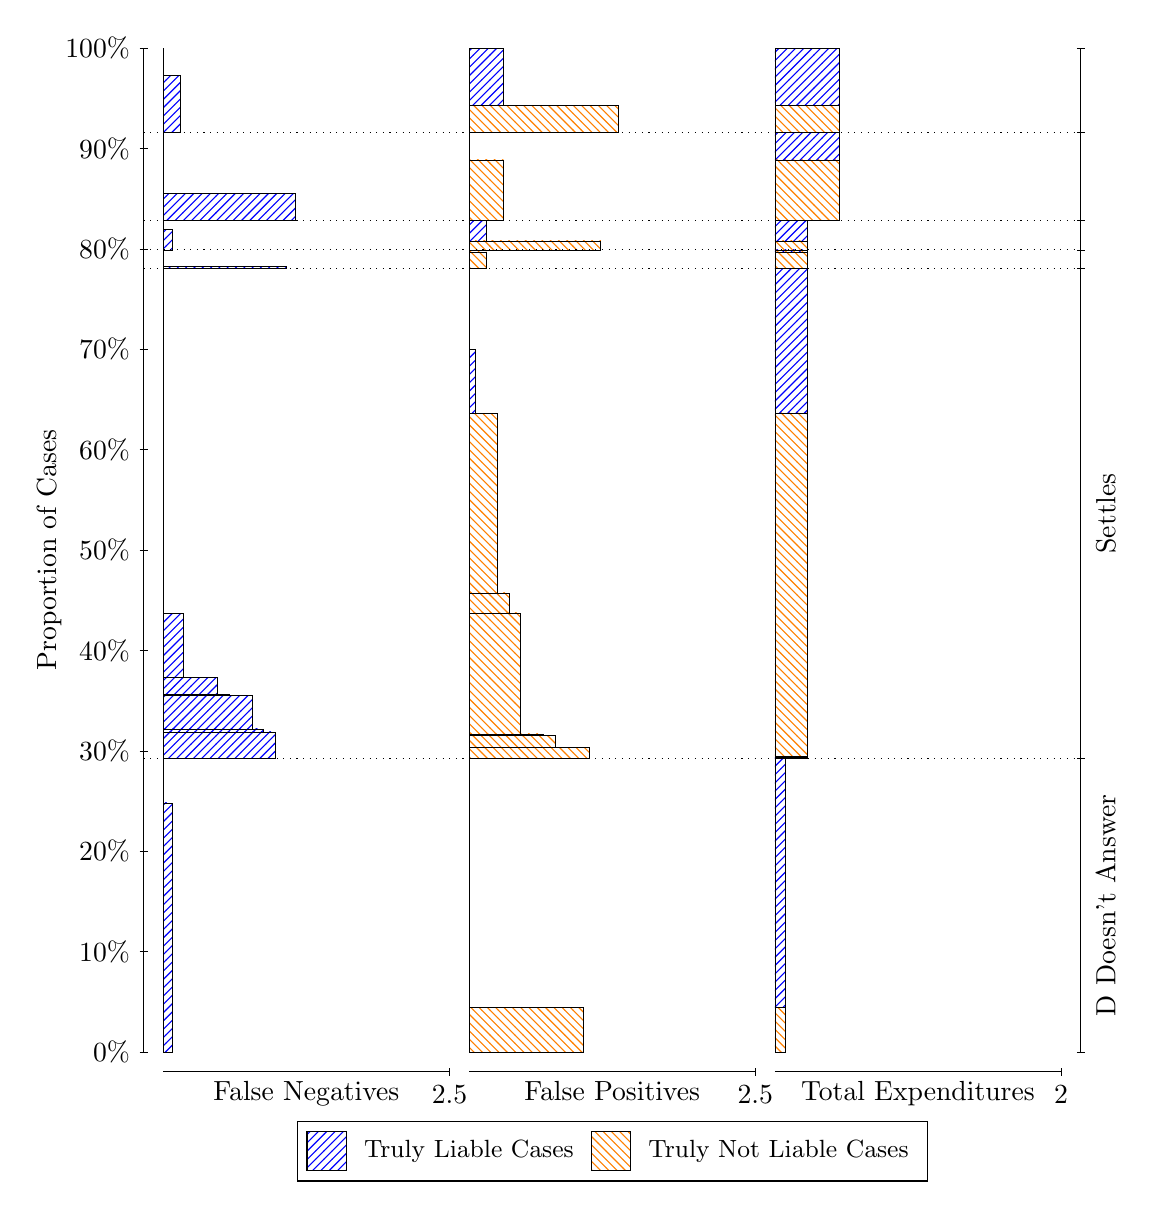
\begin{tikzpicture}
\draw[black, very thin] (1.5,1.75) -- (1.5,14.5);
\node[rotate=90, text=black, anchor=center] at (0.3, 8.125) {Proportion of Cases};
\draw[black, very thin] (1.45,1.75) -- (1.55,1.75);
\node[text=black, anchor=east] at (1.45, 1.75) {0\%};
\draw[black, very thin] (1.45,3.025) -- (1.55,3.025);
\node[text=black, anchor=east] at (1.45, 3.025) {10\%};
\draw[black, very thin] (1.45,4.3) -- (1.55,4.3);
\node[text=black, anchor=east] at (1.45, 4.3) {20\%};
\draw[black, very thin] (1.45,5.575) -- (1.55,5.575);
\node[text=black, anchor=east] at (1.45, 5.575) {30\%};
\draw[black, very thin] (1.45,6.85) -- (1.55,6.85);
\node[text=black, anchor=east] at (1.45, 6.85) {40\%};
\draw[black, very thin] (1.45,8.125) -- (1.55,8.125);
\node[text=black, anchor=east] at (1.45, 8.125) {50\%};
\draw[black, very thin] (1.45,9.4) -- (1.55,9.4);
\node[text=black, anchor=east] at (1.45, 9.4) {60\%};
\draw[black, very thin] (1.45,10.675) -- (1.55,10.675);
\node[text=black, anchor=east] at (1.45, 10.675) {70\%};
\draw[black, very thin] (1.45,11.95) -- (1.55,11.95);
\node[text=black, anchor=east] at (1.45, 11.95) {80\%};
\draw[black, very thin] (1.45,13.225) -- (1.55,13.225);
\node[text=black, anchor=east] at (1.45, 13.225) {90\%};
\draw[black, very thin] (1.45,14.5) -- (1.55,14.5);
\node[text=black, anchor=east] at (1.45, 14.5) {100\%};

\draw[black, very thin] (13.4,1.75) -- (13.4,14.5);
\draw[black, very thin] (13.35,1.75) -- (13.45,1.75);
\node[anchor=west] at (13.35, 1.75) {};
\draw[black, very thin] (13.35,5.4762) -- (13.45,5.4762);
\node[anchor=west] at (13.35, 5.4762) {};
\draw[black, very thin] (13.35,11.704) -- (13.45,11.704);
\node[anchor=west] at (13.35, 11.704) {};
\draw[black, very thin] (13.35,11.936) -- (13.45,11.936);
\node[anchor=west] at (13.35, 11.936) {};
\draw[black, very thin] (13.35,12.313) -- (13.45,12.313);
\node[anchor=west] at (13.35, 12.313) {};
\draw[black, very thin] (13.35,13.424) -- (13.45,13.424);
\node[anchor=west] at (13.35, 13.424) {};
\draw[black, very thin] (13.35,14.5) -- (13.45,14.5);
\node[anchor=west] at (13.35, 14.5) {};

\draw[black, very thin, pattern color=blue, pattern=north east lines] (1.75,1.75) rectangle (1.859,4.9142);
\draw[black, very thin, pattern color=orange, pattern=north west lines] (1.75,4.9142) rectangle (1.75,5.4762);
\draw[black, very thin, pattern color=blue, pattern=north east lines] (1.75,5.4762) rectangle (3.167,5.816);
\draw[black, very thin, pattern color=blue, pattern=north east lines] (1.75,5.816) rectangle (3.0217,5.8544);
\draw[black, very thin, pattern color=blue, pattern=north east lines] (1.75,5.8544) rectangle (2.8763,6.2809);
\draw[black, very thin, pattern color=blue, pattern=north east lines] (1.75,6.2809) rectangle (2.5857,6.2906);
\draw[black, very thin, pattern color=blue, pattern=north east lines] (1.75,6.2906) rectangle (2.4403,6.5095);
\draw[black, very thin, pattern color=blue, pattern=north east lines] (1.75,6.5095) rectangle (2.0043,7.3224);
\draw[black, very thin, pattern color=orange, pattern=north west lines] (1.75,7.3224) rectangle (1.75,11.704);
\draw[black, very thin, pattern color=blue, pattern=north east lines] (1.75,11.704) rectangle (3.3123,11.729);
\draw[black, very thin, pattern color=orange, pattern=north west lines] (1.75,11.729) rectangle (1.75,11.936);
\draw[black, very thin, pattern color=blue, pattern=north east lines] (1.75,11.936) rectangle (1.859,12.2);
\draw[black, very thin, pattern color=orange, pattern=north west lines] (1.75,12.2) rectangle (1.75,12.313);
\draw[black, very thin, pattern color=blue, pattern=north east lines] (1.75,12.313) rectangle (3.4213,12.658);
\draw[black, very thin, pattern color=orange, pattern=north west lines] (1.75,12.658) rectangle (1.75,13.424);
\draw[black, very thin, pattern color=blue, pattern=north east lines] (1.75,13.424) rectangle (1.968,14.155);
\draw[black, very thin, pattern color=orange, pattern=north west lines] (1.75,14.155) rectangle (1.75,14.5);
\draw[black, very thin, pattern color=orange, pattern=north west lines] (5.6333,1.75) rectangle (7.0867,2.312);
\draw[black, very thin, pattern color=blue, pattern=north east lines] (5.6333,2.312) rectangle (5.6333,5.4762);
\draw[black, very thin, pattern color=orange, pattern=north west lines] (5.6333,5.4762) rectangle (7.1593,5.622);
\draw[black, very thin, pattern color=orange, pattern=north west lines] (5.6333,5.622) rectangle (6.7233,5.7701);
\draw[black, very thin, pattern color=orange, pattern=north west lines] (5.6333,5.7701) rectangle (6.578,5.7886);
\draw[black, very thin, pattern color=orange, pattern=north west lines] (5.6333,5.7886) rectangle (6.2873,7.3277);
\draw[black, very thin, pattern color=orange, pattern=north west lines] (5.6333,7.3277) rectangle (6.142,7.5796);
\draw[black, very thin, pattern color=orange, pattern=north west lines] (5.6333,7.5796) rectangle (5.9967,9.858);
\draw[black, very thin, pattern color=blue, pattern=north east lines] (5.6333,9.858) rectangle (5.706,10.671);
\draw[black, very thin, pattern color=blue, pattern=north east lines] (5.6333,10.671) rectangle (5.6333,11.704);
\draw[black, very thin, pattern color=orange, pattern=north west lines] (5.6333,11.704) rectangle (5.8513,11.911);
\draw[black, very thin, pattern color=blue, pattern=north east lines] (5.6333,11.911) rectangle (5.6333,11.936);
\draw[black, very thin, pattern color=orange, pattern=north west lines] (5.6333,11.936) rectangle (7.3047,12.05);
\draw[black, very thin, pattern color=blue, pattern=north east lines] (5.6333,12.05) rectangle (5.8513,12.313);
\draw[black, very thin, pattern color=orange, pattern=north west lines] (5.6333,12.313) rectangle (6.0693,13.08);
\draw[black, very thin, pattern color=blue, pattern=north east lines] (5.6333,13.08) rectangle (5.6333,13.424);
\draw[black, very thin, pattern color=orange, pattern=north west lines] (5.6333,13.424) rectangle (7.5227,13.769);
\draw[black, very thin, pattern color=blue, pattern=north east lines] (5.6333,13.769) rectangle (6.0693,14.5);
\draw[black, very thin, pattern color=orange, pattern=north west lines] (9.5167,1.75) rectangle (9.6529,2.312);
\draw[black, very thin, pattern color=blue, pattern=north east lines] (9.5167,2.312) rectangle (9.6529,5.4762);
\draw[black, very thin, pattern color=orange, pattern=north west lines] (9.5167,5.4762) rectangle (9.9254,5.4947);
\draw[black, very thin, pattern color=blue, pattern=north east lines] (9.5167,5.4947) rectangle (9.9254,5.5045);
\draw[black, very thin, pattern color=orange, pattern=north west lines] (9.5167,5.5045) rectangle (9.9254,9.8677);
\draw[black, very thin, pattern color=blue, pattern=north east lines] (9.5167,9.8677) rectangle (9.9254,11.704);
\draw[black, very thin, pattern color=orange, pattern=north west lines] (9.5167,11.704) rectangle (9.9254,11.911);
\draw[black, very thin, pattern color=blue, pattern=north east lines] (9.5167,11.911) rectangle (9.9254,11.936);
\draw[black, very thin, pattern color=orange, pattern=north west lines] (9.5167,11.936) rectangle (9.9254,12.05);
\draw[black, very thin, pattern color=blue, pattern=north east lines] (9.5167,12.05) rectangle (9.9254,12.313);
\draw[black, very thin, pattern color=orange, pattern=north west lines] (9.5167,12.313) rectangle (10.334,13.08);
\draw[black, very thin, pattern color=blue, pattern=north east lines] (9.5167,13.08) rectangle (10.334,13.424);
\draw[black, very thin, pattern color=orange, pattern=north west lines] (9.5167,13.424) rectangle (10.334,13.769);
\draw[black, very thin, pattern color=blue, pattern=north east lines] (9.5167,13.769) rectangle (10.334,14.5);
\draw[black, dotted] (1.5,5.4762) -- (13.4,5.4762);
\draw[black, dotted] (1.5,11.704) -- (13.4,11.704);
\draw[black, dotted] (1.5,11.936) -- (13.4,11.936);
\draw[black, dotted] (1.5,12.313) -- (13.4,12.313);
\draw[black, dotted] (1.5,13.424) -- (13.4,13.424);
\draw[black, very thin] (1.75,1.5) -- (5.3833,1.5);
\node[text=black, anchor=north] at (3.5667, 1.5) {False Negatives};
\draw[black, very thin] (5.3833,1.45) -- (5.3833,1.55);
\node[text=black, anchor=north] at (5.3833, 1.45) {2.5};

\draw[black, very thin] (5.6333,1.5) -- (9.2667,1.5);
\node[text=black, anchor=north] at (7.45, 1.5) {False Positives};
\draw[black, very thin] (9.2667,1.45) -- (9.2667,1.55);
\node[text=black, anchor=north] at (9.2667, 1.45) {2.5};

\draw[black, very thin] (9.5167,1.5) -- (13.15,1.5);
\node[text=black, anchor=north] at (11.333, 1.5) {Total Expenditures};
\draw[black, very thin] (13.15,1.45) -- (13.15,1.55);
\node[text=black, anchor=north] at (13.15, 1.45) {2};

\node[text=black, centered, rotate=90] at (13.72, 3.6131) {D Doesn't Answer};
\node[text=black, centered, rotate=90] at (13.72, 8.5902) {Settles};





\draw (7.449999999999999,1.5) node[draw=none] (baseCoordinate) {};
\begin{scope}[align=center]
        \matrix[scale=0.5, draw=black, below=0.5cm of baseCoordinate, nodes={draw}, column sep=0.1cm]{
            \node[rectangle, draw, minimum width=0.5cm, minimum height=0.5cm, pattern color=blue, pattern=north east lines] {}; &
            \node[draw=none, font=\small, text=black] (B) {Truly Liable Cases}; &
            \node[rectangle, draw, minimum width=0.5cm, minimum height=0.5cm, pattern color=orange, pattern=north west lines] {}; &
            \node[draw=none, font=\small, text=black] (B) {Truly Not Liable Cases}; \\
            };
\end{scope}

\end{tikzpicture}
\end{document}